
\section{Solution}

Zum Ausführen der jeweiligen cpp Dateien muss in der Makefile die Variale \textit{Ex} auf die jeweilige Aufgabe (Ex = Ex1 oder Ex = Ex2) gesetzt werden.


\subsection{Ex 1} % (fold)
\label{sub:Ex 1}

Zum Bestimmen der Eigenwerte (Ev) wird die Funktion ".eigenvalues()" verwendet. 

Für die Potenzmethode wird ein Startvektor von $v_0 = (2,2,2,2)^T$ gewählt. Es wird $N=15$ mal iteriert.
In Tabelle \ref{tab:vergleich} sind die jeweiligen Eigenwerte dargestellt. Der Unterschied ist ziemlich gering.

\begin{table}[h]
    
    \centering
    \caption{Laufzeiten bei zwei verschieden Matrizen-Größen.}
    \sisetup{table-format=2.5}
    \begin{tabular}{S S}
        \toprule
        {\text{Eigen}} & {\text{Potenzmethode}}\\
        \midrule
        12.0851 &12.0835\\
        -9.27794 &-9.28001\\
        4.59705 &4.59705\\
        2.59583 & 2.59583\\
        
        \bottomrule
    \end{tabular}

    \label{tab:vergleich}
\end{table}

% subsection Ex 1 (end)


\subsection{Ex 2} % (fold)
\label{sub:Ex 2}

Zu Anfang wird die Matrix $A$ erstellt. 
Alle Ergebnisse sind in csv-Dateien im build-Ordner.

\begin{itemize}
    \item[a)]
    Die Matrix $A$ wird auf Tridiagonalgestalt ("Tri.csv") gebracht. Es lässt sich eine Tridiagonalgestalt erkennen. 
    Die restlichen Einträge sind zwar nicht gleich $0$, aber meist im Bereich $10^{-15}$ und damit vernachlässigbar (Maschinengenauigkeit).

    

    \item[b)]
    Nun werden die Eigenwerte bestimmt. Da die Householder-Transformation eine Ähnlichkeitstransformation ist, bleiben die Eigenwerte erhalten.
    Es wird also die Tridiagonalgestalt von Matrix $A$ verwendet, um mittels einer QR-Zerlegung die Eigenwerte zu bestimmen.
    In der QR-Zerlegung wird die Matrix in Diagonalform gebracht. Auf der Digonale stehen dann die Eigenwerte.
    Leider gelingt uns das hier nicht sehr gut. Die Matrix hat nach $N$ Iterationen weiterhin nicht zu vernachlässigende Nebendiagonalelemente.
    Diese sind wieder den csv-Dateien zu entnehmen.
    Es wird hier nur der Fall $N=10$ miteinander verglichen, da die Darstellung für $N=100$ etwas unübersichtlich ist. Die Aussagen bleiben aber für beide gleich.
    In Abbildung \ref{fig:vergleich} sind die Eigenwerte aufgetragen. Bei geringem Unterschied liegen die bestimmten Eigenwerte in ähnlichen Größenordnungen.

    \begin{figure}
        \centering
        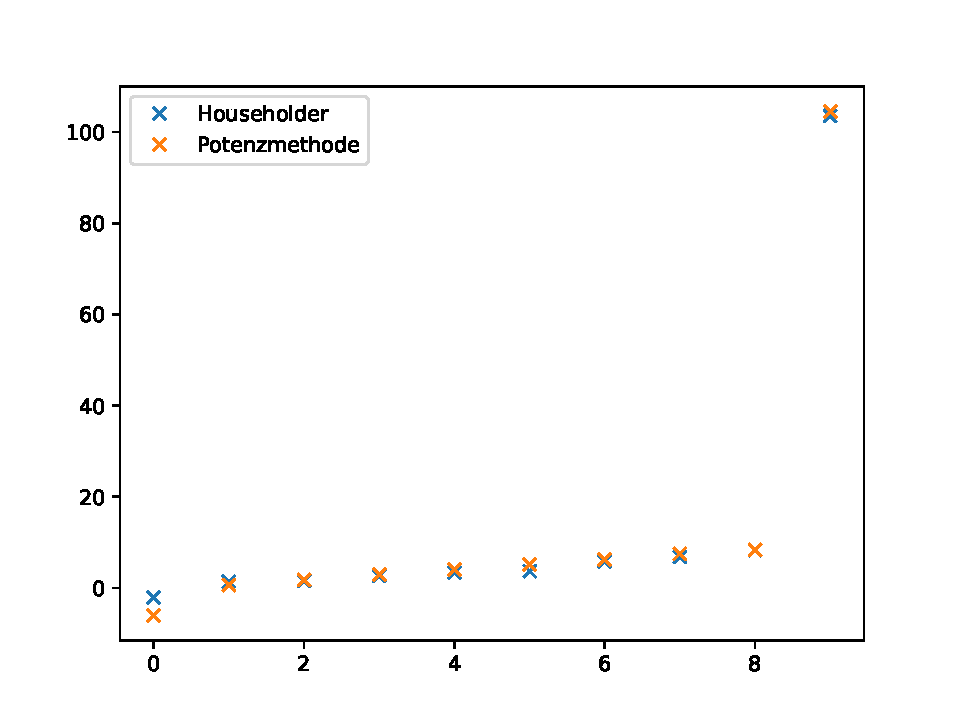
\includegraphics[width=.8\textwidth]{images/Ev_vergleich.pdf}
        \caption{Vergleich der Eigenwerte zwischen Potenzmethode und QR-Zerlegung.}
        \label{fig:vergleich}
    \end{figure}

    In Tabelle \ref{tab:Laufzeiten} sind die Laufzeiten der beiden Methoden aufgeführt.
    Leider dauert es bei uns zu lange, die Rechnung mit einer $N=1000$ Matrix durchzuführen. Alleine für $N=100$ benötigt es schon mehr als zwei Sekunden.
    Der Aufwand zur Erzeugung der Tridiagonalgestalt liegt in der Größenordnung $N^3$ und die folgende QR-Zerlegung $N^2$.
     So wird bei dem vorliegenden Code ein Laufzeitzuwachs von einem Faktor $10^3$ entstehen.

\begin{table}[h]
    \centering
    \caption{Laufzeiten bei zwei verschieden Matrizen-Größen.}
    \begin{tabular}{c c c}
        \toprule
        {$N$} & {\text{Potenzmethode}} & {\text{QR-Zerlegung}}\\
        \midrule
        10 & \qty{1.5625e-8}{\s} & \qty{0.0156}{\s} \\
        100 & \qty{2.14062e-6}{\s} & \qty{2.1406}{\s} \\
        \bottomrule
    \end{tabular}
    
    \label{tab:Laufzeiten}
\end{table}


\end{itemize}

